\documentclass{beamer}
% For more themes, color themes and font themes, see:
% http://deic.uab.es/~iblanes/beamer_gallery/index_by_theme.html
\mode<presentation>

    \usetheme{Szeged}
    \usecolortheme{whale}
    \usefonttheme{default}
    \setbeamertemplate{navigation symbols}{}
    \setbeamertemplate{caption}[numbered]
    % \setbeamertemplate{footline}[frame number]


\usepackage[english]{babel}
\usepackage[utf8x]{inputenc}
\usepackage{xcolor, graphicx,amsmath}
\usepackage[absolute,overlay]{textpos}
\title{Analogous CPU Project}
% Used on title page and each other page as well
\author{\textbf{Matthew C. Lindeman}}
\institute{\textbf{New Mexico Institute of Mining and Technology}}
\date{\textbf{\today}}

\setbeamerfont{title}{size=\LARGE,series=\bfseries,parent=structure}
\setbeamerfont{author}{size=\normalsize,series=\bfseries,parent=structure}
\setbeamerfont{institute}{size=\normalsize,series=\bfseries,parent=structure}
\setbeamerfont{date}{size=\scriptsize,series=\bfseries,parent=structure}



\begin{document}

\begin{frame}
    \titlepage
\end{frame}

\section{Introduction}
  \begin{frame}{Project Overview}
    \begin{itemize}
      \item Analogous Virtual CPU
      \item ``On the fly" scheduler implementation and testing
    \end{itemize}
  \end{frame}

  \begin{frame}{Scheduling Algorithm Interface}
    \begin{itemize}
      \item Proprietary - Good Luck
      \item FOSS Alternatives
        \begin{itemize}
          \item BSD Kernel
          \item Linux Kernel
        \end{itemize}
    \end{itemize}
  \end{frame}

  \begin{frame}{Serious Look at Linux Kernel}
    \textbf{Pros:}
    \begin{itemize}
      \item End user ease of access
      \item Personal/Enterprise Hardware Improvements
    \end{itemize}
    \textbf{Cons:}
    \begin{itemize}
      \item \textbf{\textit{TIME}}
        \begin{enumerate}
          \item 13 files entirely re-written
          \item All files that interacted with current scheduling need
            updated/new data ports
          \item Older Version (2.6.3)? (Lottery Scheduler for the Linux Kernel,
            Mejia, Morales-Betancourt, Patki)
        \end{enumerate}
      \item Inheritance From First Process
    \end{itemize}
  \end{frame}

  \begin{frame}{Decided Upon Solution}
    Make an integrated analogous virtual CPU.
  \end{frame}

\section{Analogous CPU Project}
  \begin{frame}{Preconditions and Postconditions}
    Expected input:
    \begin{itemize}
      \item A Process List
      \item A CPU
      \item Scheduling Algorithm and Related Data Structures
    \end{itemize}
    Project's Desired Output:
    \begin{itemize}
      \item Performance Statistics Such as:
        \begin{enumerate}
          \item Average rate of completion with respect to all classes of
            processes (such as memory access and IO)
          \item Total Memory Consumption
          \item etc.
        \end{enumerate}
    \end{itemize}
  \end{frame}

  \begin{frame}{Basis Of Stochastic Scheduling Algorithm}
    A basis for a stochastic scheduling algorithm must have the following
    formally:
    \begin{enumerate}
      \item $\alpha$ - The hardware on which the algorithm will run.
      \item $\beta$ - The data structures that the processes have relating them
        to the scheduling algorithm (can be the empty set!)
      \item $\gamma$ - The implementation of the scheduling of the list of
        processes (the algorithm itself).
    \end{enumerate}
  \end{frame}

  \begin{frame}{Ideal Requirements of Analgous CPU}
    \begin{itemize}
      \item Be opaque to the user with respect to anything other than the scheduling
        algorithm interface and data structure (i.e. the user can implement
        $\gamma$ without worrying about other environmental factors).
      \item Have a full list of parameters for the user to test that would
        impact the way processes are fed into the virtual CPU.
    \end{itemize}
  \end{frame}

\section{Implemented Alagous CPU System}
  \begin{frame}{Overview}
    \begin{enumerate}
      \item Compare Fair Scheduling and Lottery Scheduling Algorithms
      \item Variable Parameters
      \item Analogous $\implies$ reduction of dimension in some manner.  Here we
        just treat work/memory partitions as scalars not vectors.
    \end{enumerate}
  \end{frame}

  \subsection{Sub-System Design}
    \begin{frame}{Process}
      \begin{enumerate}
        \item Encourages Genericity With \\
          Respect to CPU/Scheduling \\
          Algorithm
        \item Process List only requires \\
          Scheduling Data Type and a \\
          max size
      \end{enumerate}
      \begin{textblock*}{2.5cm}(7cm,2.2cm)
        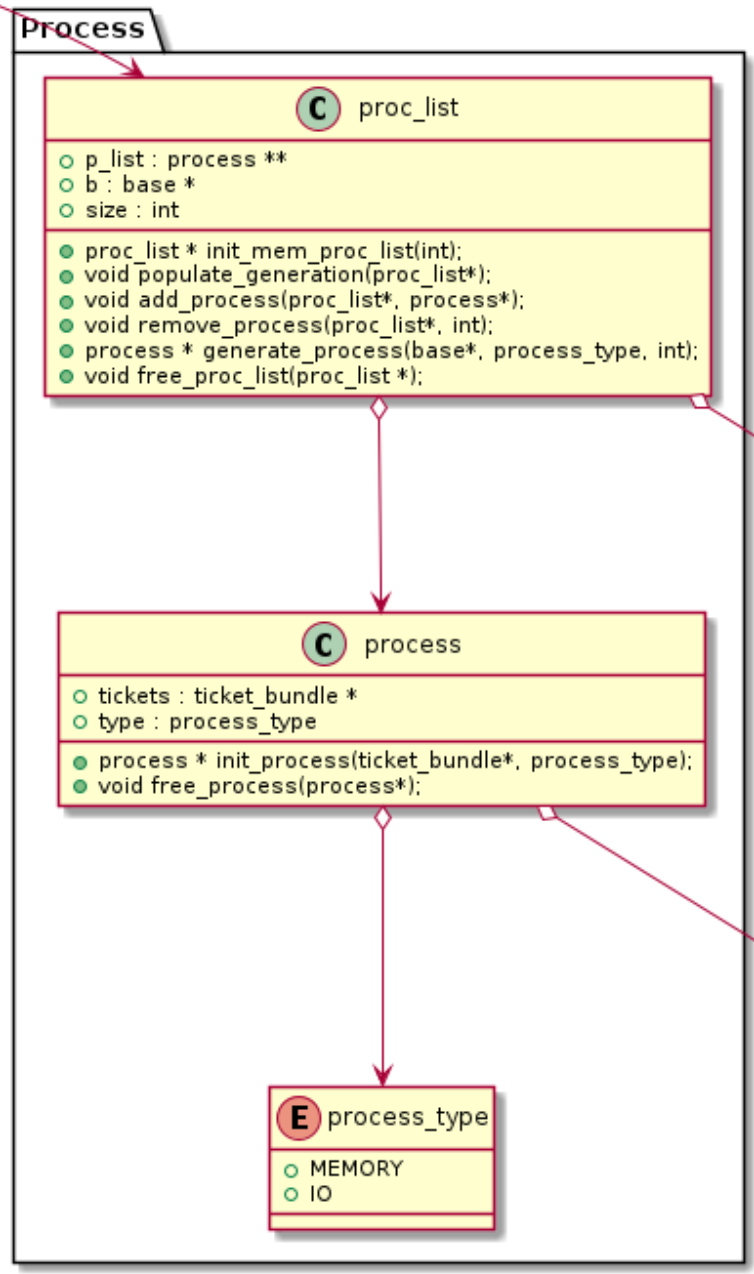
\includegraphics[scale=0.13]{{./figures/process_subsystem.png}}
      \end{textblock*}
    \end{frame}

    \begin{frame}{CPU}
      \begin{enumerate}
        \item Interfaces only with a \\
          generic scheduling algorithm \\
          and process list.
        \item Worth Noting Here Thread \\
          completion quantity per time \\
          per time quantum is a \textbf{scalar}
      \end{enumerate}
      \begin{textblock*}{2.5cm}(7cm,2.2cm)
        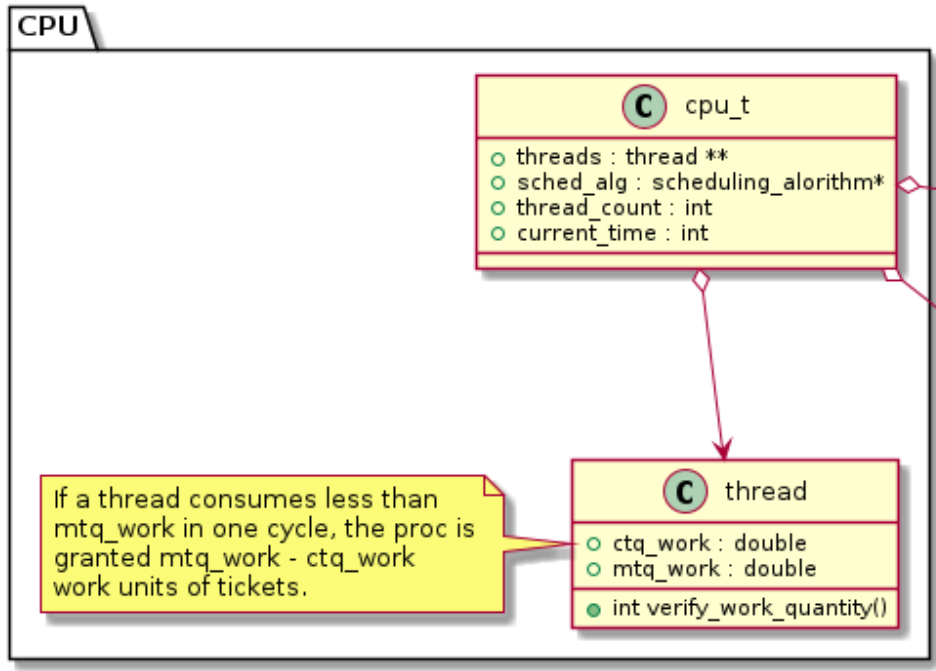
\includegraphics[scale=0.13]{{./figures/cpu_subsystem.png}}
      \end{textblock*}
    \end{frame}

    \begin{frame}{Scheduling Specific}
      \begin{enumerate}
        \item An example structure \\
          of how a user would implement \\
          an algorithm to work with the \\
          CPU simulator.
        \item  $\exists$ universal collective data \\
          structure to interface with \\
          proc$\_$list
        \item $\exists$ sub-structure for each process \\
          to point to (make SA opaque to \\
          the user!)
      \end{enumerate}
      \begin{textblock*}{2.5cm}(7cm,2.2cm)
        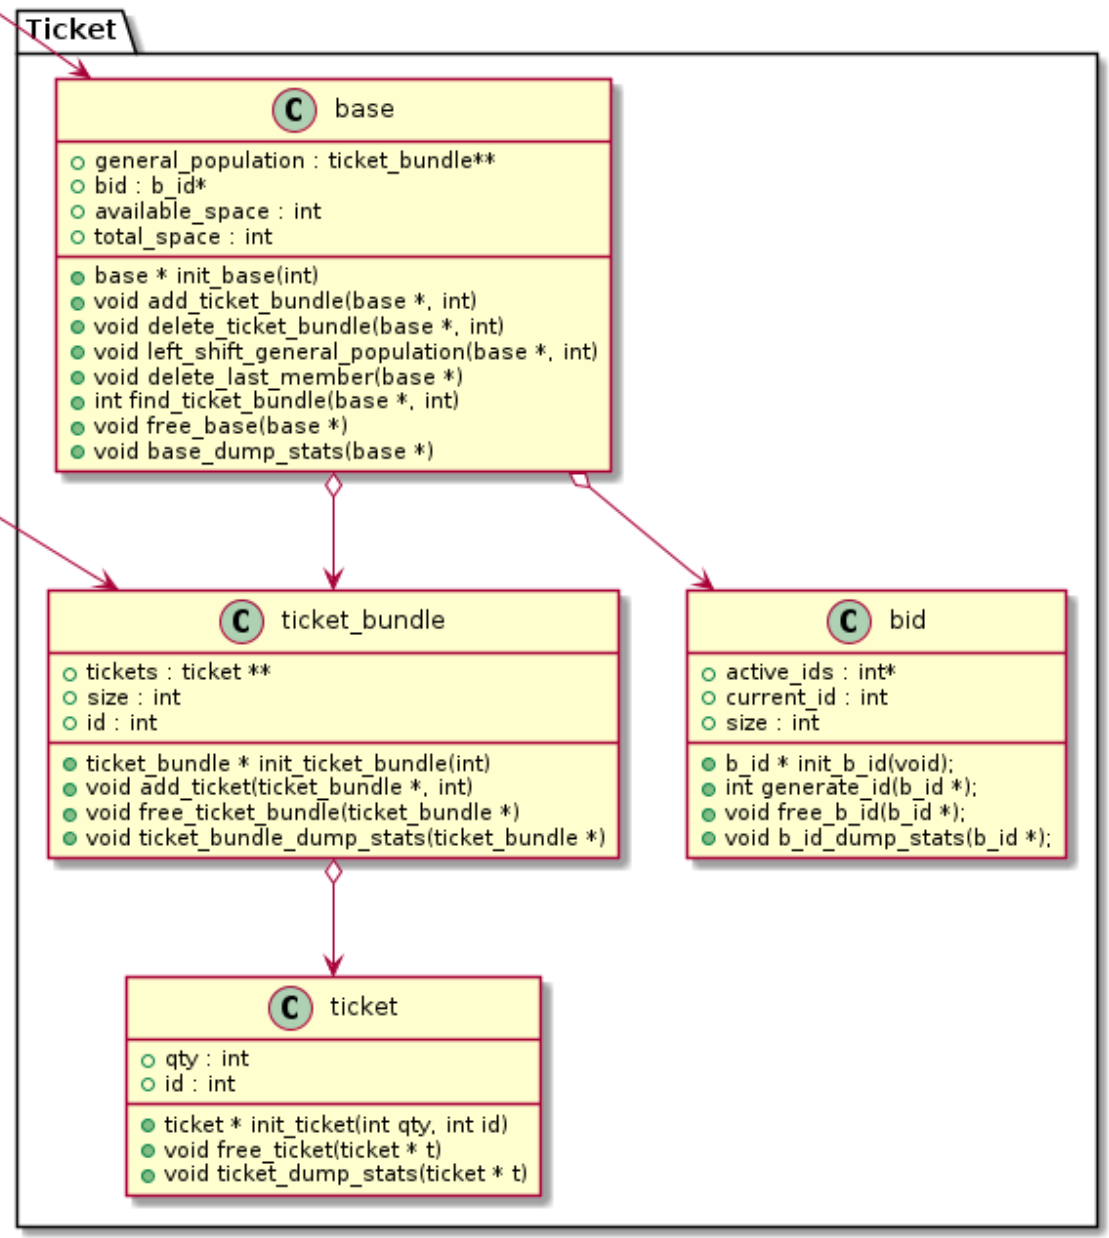
\includegraphics[scale=0.13]{{./figures/ticket_subsystem.png}}
      \end{textblock*}
    \end{frame}
  \subsection{Current Project}
    \begin{frame}{Details about Status of Project}
      This tool is still in development. The CPU, Process List, Lottery
      Scheduling data structures and most logic for the lottery scheduler are
      implemented.
      \begin{itemize}
        \item Currently a primitive working ecosystem.
        \item Data - the lottery scheduler itself still fails some unit tests
          thus the data produced cannot be trusted 100$\%$ and is not included
          here.
        \item Hosted: https://github.com/millipedes/Scheduling-Simulator/
        \item Lang: C
        \item Scope $\approx$ 1000 lines of code across 25 files.
      \end{itemize}
    \end{frame}

    \begin{frame}{Potential Future Research Potential}
      \begin{enumerate}
        \item Extensibility With Respect to Scheduling Algorithms.
        \item Additional differentiations to make between process. Such as user
          space/kernel space explicit differentiation.
        \item Implementation of opaque data statistics recording engine.
      \end{enumerate}
    \end{frame}

\end{document}
